\newpage
\section{Appendix}
\subsection{Tabular Integration by Parts}
\label{appendix:parts}
    One can use a table to perform repeated integration by parts quickly. Suppose, such as when finding the adjoint operator, we would like to use integration by parts to change the integral of \(u(x)v(x)\) into boundary terms plus the integral of \(u^{(n)}(x)v_{(n)}(x)\). Here, \(u^{(n)}\) is the \(n\)th derivative of \(u\), and \(v_{(n)}\) is the \(n\)th antiderivative of \(v\). We create a table with alternating signs in the first column, beginning with positive. In the second column, we write \(u(x)\) and its derivatives beneath it while alternating the sign. In the third column, we write \(v(x)\) and its anti-derivatives beneath it. 
    Next, we take the \(i^{\mathrm{th}}\) sign in the left column to be the sign of \(u^{(i)}\), multiply diagonal terms, and add each product.
    These are the boundary terms. Lastly, we multiply the bottom terms together, which becomes the integrand. 
    \begin{figure}[H]
        \centering
        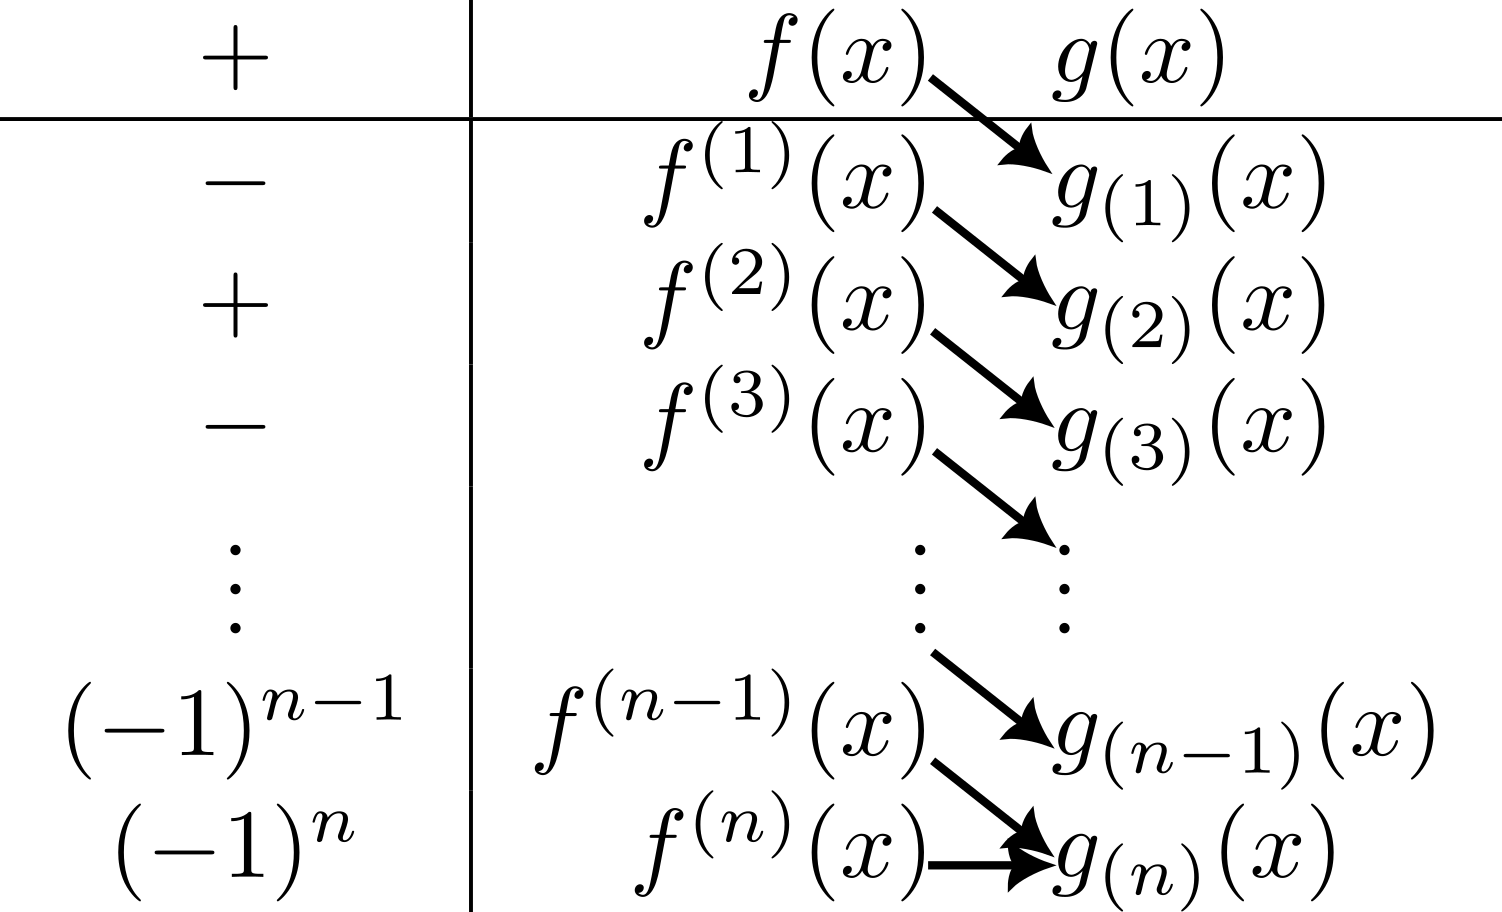
\includegraphics[width=0.34\linewidth]{include/tabular-boundary.png}
    \end{figure}
    At the end of this process, the original integral has become 
    % \begin{equation*}
    %     \begin{split}
    %         \intl u(x)v(x) dx &= (u(x)v_{(1)}(x)-u^{(1)}(x)v_{(2)}(x)+u^{(2)}(x)v_{(3)}(x) + \cdots + (-1)^{n-1} u^{(n-1)}(x))\biggr\rvert_\mathrm{a}^\mathrm{b}\\ &+ \intl v^{(4)}(x)u(x) dx.
    %     \end{split}
    % \end{equation*}
    \begin{equation*}
        \begin{split}
            \intl u(x)v(x) dx &= \left(\sum_{i=1}^{n} (-1)^{i-1}u^{(i-1)}(x)v_{(i)}(x)\right)\biggr\rvert_\mathrm{a}^\mathrm{b} + (-1)^n\intl u^{(n)}(x)v_{(n)}(x) dx.
        \end{split}
    \end{equation*}
\subsection{The Mean Value Theorem}
    The mean value theorem for integration states that for any function \(f\) which is integrable on \([a,b]\), there exists a value \(c\) where \(a < c < b\) such that
    \begin{equation*}
        \int_{a}^{b} f'(x)dx = f'(c)(b-a).
    \end{equation*}
\subsection{Big O Notation} \label{sec:BigO}
Big O notation is used to describe the limiting behavior of a function as the argument tends to some value or plus or minus infinity. By \(f(x)=O(g(x))\) as \(x\to x_0\) we mean that \(\frac{f(x)}{g(x)}\) is bounded as \(x\to x_0\). For example 
\begin{equation*}
    \sin 6x = O(1) \text{ as } x\to \inf.
\end{equation*}

\subsection{Alternative Method of Green's Functions}
In this text, we approach finding the Green's function by finding the adjoint operator and then defining 
\begin{equation*}
    \Lstar G = \d(\x-x).
\end{equation*}
Instead, one can find an alternative version of the Green's function, which we denote by \(G^*\), using the original differential operator acting on \(u\). 

Suppose a differential equation is given by
\begin{equation*}
    \L_x u = \phi.
\end{equation*}
We can define \(G^*(\xi,x)\) to be a function that satisfies,
\begin{equation*}
    \L_x G^* = \d(\x-x).
\end{equation*}
Consider
\begin{equation*}
    u(x) = \intl G^*(\x,x)\phi(\x)d\x.
\end{equation*}
Assuming \(G^*\) may be chosen so that the boundary conditions are satisfied,
\begin{equation*}
    \begin{split}
        \L_x u &= \L_x \intl G^*(\x,x)\phi(\x)d\x\\ 
        &= \intl \L_xG^*(\x,x)\phi(\x)d\x  \\ 
        &= \intl \d(\x-x)\phi(x)dx\\  
        &= \phi(x)
    \end{split}
\end{equation*}
so long as the equation \(\L_x\int = \int \L_x\) may be justified.
